\documentclass[paper=a4, fontsize=12pt]{scrartcl}
\usepackage{graphicx}
\usepackage[protrusion=true,expansion=true]{microtype}
\usepackage{amsmath,amsfonts,amsthm}
\usepackage{fourier}
\usepackage[utf8]{inputenc}
\usepackage{amsmath}
\usepackage{amsfonts}
\usepackage{amssymb}
\usepackage[OT4]{fontenc}
\usepackage[polish]{babel}
\usepackage{epstopdf}
\usepackage{fancyhdr}
\usepackage{hyperref}
\pagestyle{fancyplain}
\fancyhead{}	
\renewcommand{\headrulewidth}{1pt}
\renewcommand{\footrulewidth}{1pt}
\textheight = 700pt
\textwidth = 500pt
\hoffset =-30pt
\begin{document}
\begin{flushright}
03.03.2016 r.\\
dr Robert Bryl
\end{flushright}Paweł Grabiński\\
Rok 3, Fizyka teoretyczna\\[0.5cm]
{\huge \bf Wyznaczanie ładunku właściwego elektronu}
\section{Wyniki}
W przeprowadzonym doświadczeniu uzyskaliśmy następujące wyniki:
\begin{itemize}
	\item Metoda pola podłużnego: $\frac{e}{m}=(1.550\pm0.014)\cdot10^{11}\:\mathrm{\frac{C}{kg}}$
	\item Metoda poprzecznego pola elektrycznego: $\frac{e}{m}= (2.085\pm0.037)\cdot10^{11}\:\mathrm{\frac{C}{kg}}$
	\item Metoda poprzecznego pola magneytcznego: $\frac{e}{m}=(1.140\pm0.055)\cdot10^{11}\:\mathrm{\frac{C}{kg}}$
	\item Metoda Thompsona: $\frac{e}{m}= (1.539\pm0.016)\cdot10^{11}\:\mathrm{\frac{C}{kg}}$
\end{itemize}
\section{Tabela pomiarowa}
\subsection{Przypadek pola podłużnego}
\begin{align*}
L=0.457\:\mathrm{m} \qquad \Delta L=0.001 \:\mathrm{m} \qquad N_s=510 
\end{align*}
\begin{table}[h]
	\begin{tabular}{|l|l|l|l|l|l|l|l|l|l|l|l|l|l|}
		\hline
		$U\:[\mathrm{V}]$ & 300  & 400  & 500  & 600  & 700  & 800  & 900  & 1000 & 1100 & 1200 & 1300 & 1400 & 1500 \\ \hline
		$I_1\:[\mathrm{A}]$ & 3.38 & 3.98 & 4.55 & 5.11 & 5.37 & 5.78 & 6.22 & 6.41 & 6.78 & 7.05 & 7.45 & 7.69 & 8.11 \\ \hline
		$I_2\:[\mathrm{A}]$ & 2.99 & 3.17 & 3.60 & 3.92 & 4.20 & 4.55 & 4.82 & 5.11 & 5.42 & 5.68 & 5.83 & 5.97 & 6.34 \\ \hline
	\end{tabular}
\end{table}
\subsection{Przypadek pola poprzecznego	}
\begin{table}[h]
	\begin{tabular}{|l|l|l|l|l|l|l|l|l|}
		\hline
		$d\:[0.005\:\mathrm{m}]$ & -4    & -3    & -2    & -1   & 1    & 2     & 3     & 4    \\ \hline
		$U\:[\mathrm{V}]$ & 46.25 & 33.75 & -23   & 10   & 10.5 & 22    & 32.5  & 42.5 \\ \hline
		$I\:[\mathrm{mA}]$ & 51.25 & 37.5  & 26.25 & 12.5 & 15   & 26.25 & 38.75 & 52.5 \\ \hline
	\end{tabular}
\end{table}
\subsection{Metoda Thompsona}
\begin{table}[h]
	\begin{tabular}{|l|l|l|l|l|l|l|l|l|}
		\hline
		$d\:[0.005\:\mathrm{m}]$ & -4    & -3    & -2 & -1    & 1    & 2    & 3    & 4     \\ \hline
		$U\:[\mathrm{V}]$ & 43.75 & 33.75 & 22 & 10.25 & 10.5 & 21.5 & 32.5 & 42.5  \\ \hline
		$I\:[\mathrm{mA}]$ & 53.75 & 38.75 & 25 & 13    & 13.5 & 26   & 42.5 & 58.75 \\ \hline
	\end{tabular}
\end{table}
\section{Opis teoretyczny}
\subsection{Nierelatywistyczny ruch cząstki naładowanej w polu elektromagnetycznym}
Pole elektromagnetyczne jest zadane dwoma wektorami - wektorem natężenia pola elektrycznego  oraz indukcji pola magnetycznego.\\
Pole elektromagnetycze działa na cząstkę tzw. siłą Lorentza[2]:
\begin{align}
\vec{F}=q\vec{E}+q\vec{v}\times\vec{B}
\end{align}
\subsubsection{Jednorodne pole elektryczne}
Stałe jednorodne pole elektryczne przyspiesza cząstke, a wskutek działania siły elektrostatycznej cząstka będzie się odchylała i poruszała się po gałęzi paraboli. Równaniem jej ruchu będzie więc równanie ruchu jednostajnego z przyspieszeniem:
\begin{align}
\vec{r}=\vec{r}_0+\vec{v_0}t-\frac{et^2}{2m}\vec{E}
\end{align}
W szczególnym przypadku, gdy prędkość będzie skierowana wzdłuż kierunku pola, ruch zachodzi po prostej.
\subsubsection{Jednorodne pole magnetyczne}
Stałe jednorodne pole magnetyczne. W tym przypadku mamy do rozwiązania następujące równanie:
\begin{align*}
	m\vec{a}=q\vec{v}_0\times\vec{B}
\end{align*}
Ogólnym rozwiązaniem jest skośna linia śrubowa. Jeśli prędkość jest równoległa do pola, to obserwujemy ruch prostoliniowy. Jeśli prędkość jest prostopadła, to zachodzi przypadek ruchu po okręgu.
\subsubsection{Równległe jednorodne pola} 
Pola $\vec{E}$ i $\vec{B}$ skierowane są wzdłuż osi $Oz$. Rrozpiszemy powyższe równania na składowe:
\begin{align*}
m\ddot{x}=q\dot{y}B,\qquad m\ddot{y}=-q\dot{x}B, \qquad m\ddot{z}=qE
\end{align*}
Rozwiązaniem równania ruchu są postaci:
\begin{align*}
x=\frac{v_0}{\omega}\sin\omega t,\\
y=-\frac{v_0}{\omega}\cos(1-\omega t),\\
z=z_0+\dot{z}_0t-\frac{1}{2}\frac{e}{m}Et^2,\\
\omega=\frac{eB}{m}.
\end{align*}
Ruch w kierunku osi $Oz$ zachodzi niezależnie od ruchu w płaszczyźnie $Oxy$. Widzimy, że ruch jest ruchm śrubowym, przy czym w kieurnku $z$ jest to ruch jednostajnie przyspieszony.
\subsubsection{Prostopadłe jednorodne pola}
Przestudiowanie tego przypadku bardzo ułatwi nami opis zjawisk zachodzących w polu elektormagnetycznym, ponieważ zawsze możemy rozłożyć pole na składową prostopadłą i równoległą.
Niech pole $\vec{B}$ będzie skierowane wzdłuż osi $Oz$, a pole $\vec{E}$ wzdłuż osi $Oy$. Wówczas równania ruchu można zapisać w następującej postaci:
\begin{align*}
m\ddot{x}=e\dot{y}B,\qquad m\ddot{y}=-e\dot{x}B+eE, \qquad m\ddot{z}=0
\end{align*}
Rozważamy warunki początkowe:
\begin{align*}
x_0=0,\qquad y_0=0,\qquad z_0=0\\
\dot{x}_0=v_0,\qquad\dot{y}_0=0,\qquad\dot{z}_0=v_z
\end{align*}
Dostaniemy równania:
\begin{align*}
x=\frac{1}{\omega}\left(v_0-\frac{eE}{m\omega}\right)\sin\omega t+\frac{eE}{m\omega}t\\
y=\frac{1}{\omega}\left(v_0-\frac{eE}{m\omega}\right)\left(\cos\omega t - 1\right)\\
z=v_zt
\end{align*}

\subsection{Solenoid}
Solenoidem nazywamy długą cewkę, ciasno nawiniętą wzdłuż linii śrubowej. Zakładamy przy tym, że długość solenoidu jest znacznie większa od jego średnicy. Pole magnetyczne solenoidu jest superpozycją pól, wytwarzanych przez pojedyncze zwoje, z których składa się solenoid. Dla punktów położonych bardzo blisko uzwojenia, każdy zwój zachowuje się pod względem magnetycznym prawie tak, jak długi prostoliniowy przewód, a linie pola tworzą prawie współśrodkowe okręgi.
Pola między sąsiednimi zwojami niemal całkowicie sie znoszą natomiast wewnątrz solenoidu i dostatecznie daleko od uzwojenia $\vec{B}$ jest w przybliżeniu równoległy do osi solenoidu. W graniczym przypadku solenoidu idealnego, który jest nieskończenie długi i składa się ze ściśle ułożonych zwojów, pole wewnątrz solenoidu jest jednorodne i równoległe do jego osi. Kierunek możemy wyznaczyć zgodnie z regułą prawej ręki: należy wyobrazić sobie, że kładziemy na cewce dłoń tak, by cztery palce wskazywały kierunek przepływu prądu. Wtedy kciuk wskaże kierunek wektora indukcji magnetycznej - zgodny z osią solenoidu[2]. 
\begin{figure}[h]
\centering
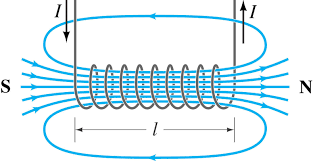
\includegraphics[width=0.5\linewidth]{sl}
\caption{Poglądowy schemat solenoidu}
\label{fig:sl}
\end{figure}

W punktach położonych powyżej osi solenoidu pole wytworzone przez górne częście solenoidu jest skierowane w lewo i częściowo się znosi z polem pochodzącym od dolnych części zwojów (leżą do siebie dostatecznie blisko, średnica cewki jest względnie mała). Dla solenoidu idealnego indukcja pola magnetycznego na zewnątrz jest równa zeru. Założenie jest spełnione, jeżeli długość solenoidu jest dużo większa od jego średnicy, a rozważany punkt,w którym badamy indykcję leży na zewnątrz solenoidu dostatecznie daleko od jego końców. 
W rzeczywistym solenoidzie w środkowym obszarze odległości między liniami pola magnetycznego są małe, co wskazuje, że pole wewnątrz cewki jest dość silne, jest również jednorodne. Na zewnątrz zaś nie znika, jak w solenoidzie idealnym, ale jest stosunkowo słabe.
Zastosujemy prawo Ampere’a do idealnego solenoidu[1]:
\begin{align*}
\oint \vec{B}\cdot d\vec{l}=\mu_0I_{tot}
\end{align*}
Jako kontur całkowania wybieramy prostokąt składający się z dwóch odcinków równoległych do pola i dwóch prostopadłych. Jeden z odcinków równoległych znajduje się wewnątrz solenoidu, a drugi poza nim. Długość odcinków równoległych wynosi $l$. Możemy całkę krążenia rozbić na cztery całki:
\begin{align*}
\int\limits_{\parallel in} \vec{B}\cdot d\vec{l}
+\int\limits_{\perp 1} \vec{B}\cdot d\vec{l}
+\int\limits_{\parallel out} \vec{B}\cdot d\vec{l}
+\int\limits_{\perp 2} \vec{B}\cdot d\vec{l} =
\mu_0 IN
\end{align*}
Całki z odcinków prostopadłych do pola wynoszą $0$. Całka z odcinka znajdującego się poza solenoidem wynosi $0$, ponieważ poza cewką $\vec{B}=0$. Jedynie zostaje nam pierwsza całka. Teraz wprowadzimy gęstość uzwojenia $n=\frac{N_{tot}}{l_{tot}}$:
\begin{align*}
Bl=\mu_0 Inl\Rightarrow B=\mu_0In
\end{align*}
Formalizm ten wyprowadzony dla solenoidu idealnego jest bardzo dobrym przybliżeniem dla solenoidu rzeczywistego, jeśli tylko zastosujemy go do punktów dostatecznie dalekich od jego końców. Wzór ten jest potwierdzony doświadczalnie, pokazuje on, że wartość indukcji pola magnetycznego wewnątrz solenoidu nie zależy od własności geometrycznych. Solenoid umożliwia nam wytwarzanie jednorodnego pola magnetycznego o zadanej wartości.
\subsection{Metody wyznaczania ładunku właściwego}
Stosunek ładunku cząstki do jej masy nazywamy ładunkiem właściwym. Istnieje kilka metod pomiarowych, służących wyznaczaniu stosunku $e/m$:
\begin{itemize}
	\item Metoda poprzecznego pola
	\item Metoda Thomsona 
	\item Metoda Buscha (podłużnego pola magnetycznego)
	\item Metoda filtru prędkości
\end{itemize}
\subsubsection{Metoda poprzecznego pola magnetycznego}  Rozważmy wiązkę elektronów, która porusza się ze stałą prędkością  w próźni w płaszczyźnie prostopadłej do kierunku wektora indukcji zewnętrznego pola magnetycznego. 
Siła przez cały czas ruchu jest skierowana prostopadle do kierunku wektora prędkości cząstki. Z założenia na cząstkę  nie działają inne siły. Zatem cząstka pod działaniem siły Lorentza porusza się po okręgu o promieniu: \begin{align*}
R=\frac{mv_0}{eB}
\end{align*}.
Promień krzywizny toru i pole mierzymy bezpośrednio. Prędkość możemy wyznaczyć z różnicy potencjałów pomiędzy anodami przyspieszającymi wiązkę:
\begin{align*}
m\frac{v_0^2}{2}=eU\Rightarrow v_0^2=2U\frac{e}{m}
\end{align*}
Łącząc te dwa wzory dostajemy wyrażenie na ładunek właściwy:
\begin{align}
\frac{e}{m}=\frac{2U}{B^2R^2}
\end{align}

\subsubsection{Metoda Thompsona}
Wiązkę cząstek naładowanych, która porusza się ze stałą prędkością  w próźni, przepuszczamy jednocześnie przez pole elektryczne i prostopadłe do niego pole elektryczne. 
\begin{figure}[h!]
\centering
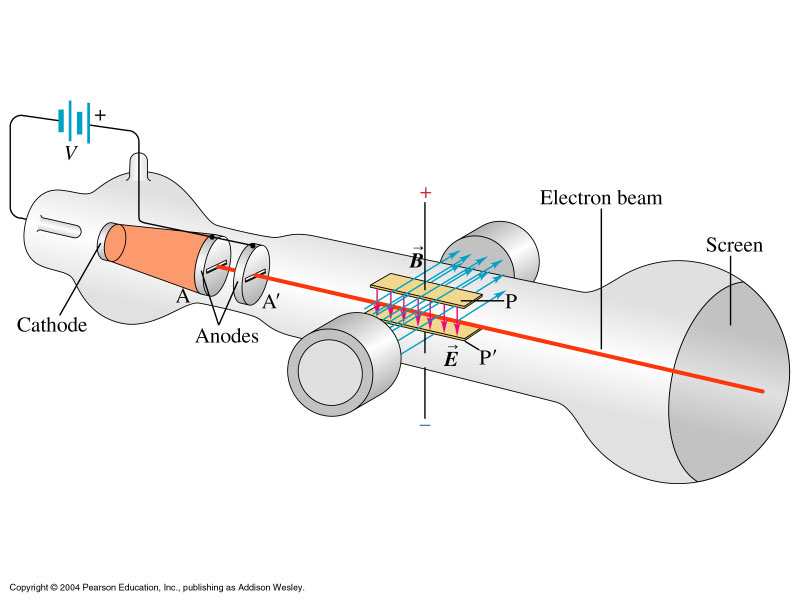
\includegraphics[width=0.5\linewidth]{thla}
\caption{Układ pomiarowy metody Thompsona}
\label{fig:thla}
\end{figure}

Katoda jest źródłem naszej wiązki. Elektrony są przyspieszane przez różnicę potnecjałów pomiędzy anodami \textbf{A} i \textbf{A'}, uzyskując pewną prędkość. W dalszej części układu wsytępują jednorodne pola elektryczne i magnetyczne. Pole elektryczne wytwarzane jest przez płytki \textbf{P} i \textbf{P'}, a pole magnetyczne przez elektromagnes.
Na końcu układu znajduje się ekran, na którym świecąca plamka określa miejsce padania wiązki.\\

W wyniku działania pola elektrycznego na cząstkę, obserwujemy przesunięcie plamki na ekranie. Z wartości przesunięcia od środka ekranu oblicza się promień krzywizny toru. Następnie, odpowiednio dobranymi wartościami prądów w obwodach, korygujemy tor wiązki, tak by padała na środek ekranu. Z warunku równoważenia się składowej elektrycznej i magntycznej siły Lorentza, możemy wyznaćzyć stosunek $e/m$.

\subsubsection{Metoda podłużnego pola magnetycznego - Buscha}
Rozważmy wiązkę elektronów, która porusza się ze stałą prędkością tworzącą niezerowy kąt z kierunkiem indukcji pola magnetycznego. By ułatwić opis, możemy podzielić prędkość na dwie składowe: równoległą  i prostopadłą do kierunku pola. \begin{align*}
v_\perp=v_0\sin\alpha\qquad v_\parallel=v_0\cos\alpha
\end{align*}  W kierunku rónoległym do pola elektron porusza się ruchem jednostajnym z prędkością $v_\parallel$. W płaszczyźnie prostopadłej do kierunku pola elektron porusza się po okręgu o promieniu $R=\frac{mv_\perp}{eB}$. Sumą tych ruchów jest linia śrubowa.\\
Okres ruchu wzdłuż linii śrubowej wynosi:
\begin{align*}
T=\frac{2\pi R}{v_\perp}
\end{align*}
Uwzględniając krzywiznę ruchu:
\begin{align*}
T=\frac{2\pi}{\frac{e}{m}B}
\end{align*}
Teraz zauważmy, że jeśli skonstrujemy układ pomiarowy tak, by w trakcie jednego okresu elektron przebywał całą długość $l$ obszaru, w którym występuje pole magnetyczne, do ekranu, to:
\begin{align*}
T=\frac{l}{v_\parallel}
\end{align*}
Inaczej mówiąc, staramy się doprowadzić do takiej sytuacji, by ognisko elektronów na ekranie znajdowało się na osi układu.\\

Ponieważ kąt odchylenia prędkości od kierunku pola jest mały, to możemy przybliżyć $\cos\alpha\approx1$. Prędkość początkową możemy wyznaczyć ponownie z różnicy potencjałów w elemencie układu przyspieszającym wiązkę:
\begin{align*}
T=\frac{l}{\sqrt{2U\frac{e}{m}}}
\end{align*}
Czyli możemy połaczyć dwa wzory na okres:
\begin{align*}
\frac{2\pi}{\frac{e}{m}B}=\frac{l}{\sqrt{2U\frac{e}{m}}}
\end{align*}
Dostajemy wzór na ładunek właściwy:
\begin{align}
\frac{e}{m}=\frac{8\pi^2U}{l^2B^2}
\end{align}
\subsubsection{Metoda filtrów prędkości}
Ponownie rozważmy wiązkę elektronów, która porusza się ze stałą prędkością  i jest przyspieszana w obszarze pola elektrycznego pomiędzy anodami. Następnie wiązka przechodzi przez dwa kondensatory płaskie. Pomiędzy kondensatorami umieszczona jest przesłona, przepuszczająca tylko te elektrony, które nie zostały odchylone w pierwszym kondensatorze. Do obu kondensatorów przykładane jest synchroniczne, zmienne w czasie napięcie sinusoidalne o okresie $T$. Wtedy przez przesłonę pomiędzy kondensatorami mogą przejść tylko te elektrony, które przeleciały przez pierwszy kondensator, gdy pole było zerowe. Po czasie $t$ elektrony lecą do drugiego kondensatora, napięcie już zostanie zmienione i elektrony się odchylą. Odchylenie nie nastąpi tylko, jeśli $t=\frac{T}{2}n$.
Wtedy wiązka da ślad w środku ekranu. By strumień nie był odchylony, musi zachodzić warunek:
\begin{align*}
t^2=\frac{l^2}{v^2},\qquad
v^2=\frac{2eU}{m},\qquad t=\frac{T}{2}n\qquad\Rightarrow\qquad
\frac{T^2}{4}n^2=\frac{l^2m}{2eU}
\end{align*}
Gdzie $l$ to odległość pomiędzy kondensatorami.\\
Końcowo ładunek właściwy:
\begin{align}
\frac{e}{m}=\frac{2l^2}{UT^2n^2}
\end{align}
W celu wykonania pomiaru okres napięcia sinusoidalnego $T$ zmniejsza się, aż wiązka elektronów  wpadnie dokładnie na środek ekranu, co odpowiada przyjętemu przez nas warunkowi. 
\subsubsection{Lampa oscyloskopowa (Brauna)}
\begin{figure}[h!]
\centering
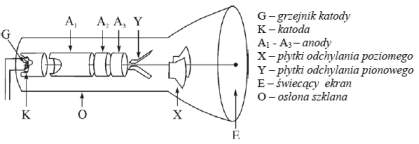
\includegraphics[width=0.6\linewidth]{lo}
\caption{Schemat budowy lampy oscyloskopowej}
\label{fig:lo}
\end{figure}
Źródłem elektronów jest żarząca katoda \textbf{K}. Wiązka pochodząca z katody przechodzi przez anody \textbf{A}, gdzie jest odpowiednio przyspieszana. Dalej wchodzi w obszar pionowego pola elektrycznego \textbf{Y}, a następnie w obszar poziomego pola \textbf{X}. Na końcu wiązka ogniskuje się na ekranie, gdzie możemy ją zobaczyć w postaci święcącej plamki.
W jednym z kondensatorów wytwarzamy pole elektryczne związane z badanym napięciem. Do okładek drugiego podłączamy napięcie drgań relaksacyjnych piłowych.
W trakcie każdego okresu napięcie pierw rośnie z czasem, a potem nagle spada do $0$. Efektem takiego napięcia jest poruszanie się plamki na ekranie ze stałą prędkością, którą możemy kontrolować.

\subsection{Cewki Helmholtza}
Cewkami Helmoholtza nazywa się układ cewek, wytwarzający w pewnym ograniczonym obszarze jednorodne pole magnetyczne.  Układ taki składa się z cewek połączonych szeregowo i ustawionych równolegle w odległości równej promieniowi każdej z nich.

\begin{figure}[h!]
\centering
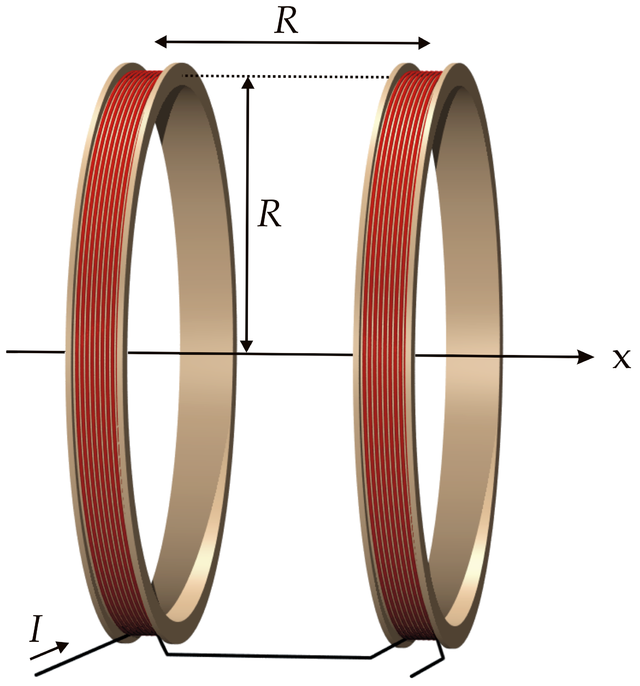
\includegraphics[width=0.3\linewidth]{ch}
\caption{Schemat Cewek Helmholtza}
\label{fig:ch}
\end{figure}

\subsubsection{Pole magnetyczne cewek Helmholtza}
\begin{figure}[h!]
\centering
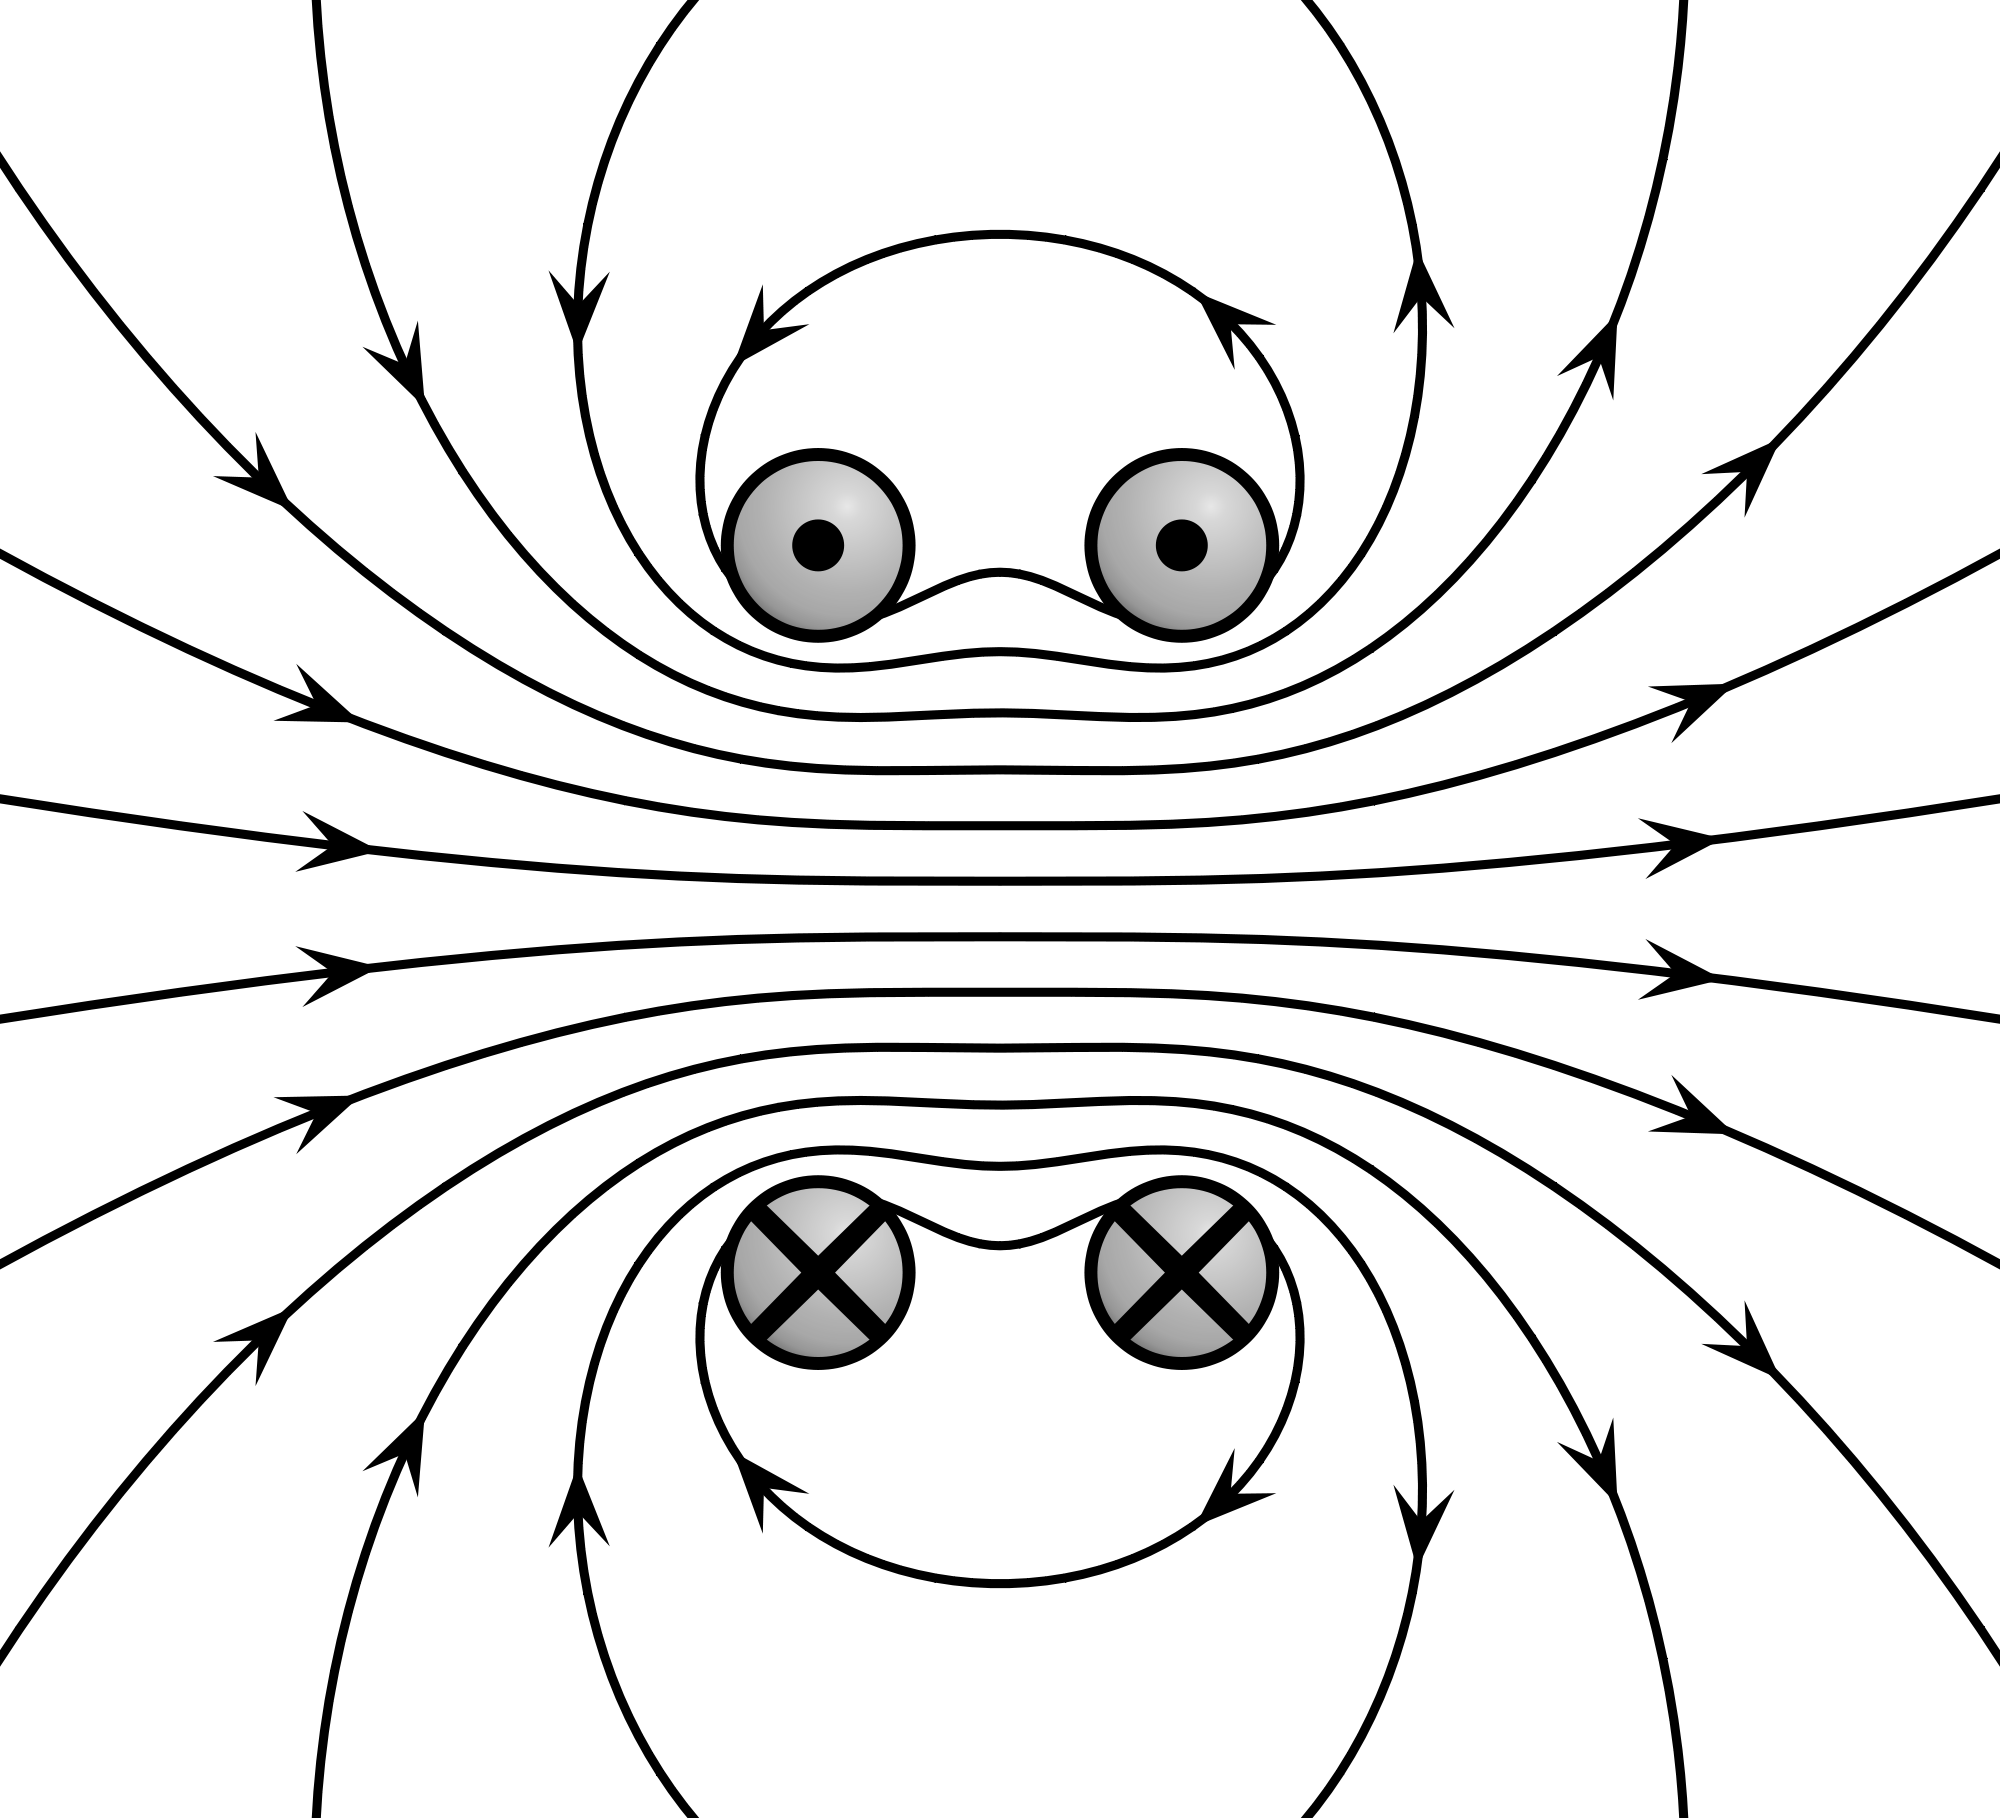
\includegraphics[width=0.3\linewidth]{chp}
\caption{Pole magnetyczne cewek Helmholtza}
\label{fig:chp}
\end{figure}

Indukcję pola magnetycznego możemy otrzymać z  prawa Biorta-Savarta[1]:
\begin{align}
\vec{B}=\frac{\mu_0}{4\pi}I\int\frac{d\vec{l}\times \hat{x}}{R^2+\vec{x}^2}
\end{align}
Gdzie:
\begin{itemize}
	\item $I$ to natężenie prądu w obwodzie cewek
	\item $\vec{x}$ to odległość od $d\vec{l}$
	\item $R$ to promień cewek oraz odległość między nimi
	\item $\mu_0$ to stała przenikalności magnetycznej próżni
\end{itemize}
Interesuje nas wartość pola równolgła do osi obrotu cewek:
\begin{align*}
B=\frac{2\pi R\mu_0nI}{4\pi (R^2+\vec{x}^2)} \frac{R}{(R^2+\vec{x}^2)^\frac{1}{2}}=
\frac{ R^2\mu_0nI}{2(R^2+\vec{x}^2)^\frac{3}{2}}
\end{align*}
Ostatecznie interesuje nas wartość dla dwóch cewek Helmoholtza w połowie odległości pomiędzy nimi $x=\frac{R}{2}$:
\begin{align}
B=2\cdot
\frac{R^2\mu_0nI}{2(R^2+\frac{R}{2}^2)^\frac{3}{2}}=
\frac{\mu_0nI}{R(\frac{5}{4})^\frac{3}{2}}=
\left(\frac{4}{5}\right)^\frac{3}{2}\frac{\mu_0nI}{R}
\end{align}
\section{Opis doświadczenia}
\subsection{Metoda pola podłużnego}
W tej metodzie wykonujemy następujące czynności:
\begin{enumerate}
\item Mierzymy długość solenoidu. Ilość zwojów jest wskazana na cewce.
\item Do płytek odchylających lampy oscyloskopowej przykładamy zmienne napięcie powodujące rozproszenie kątowe wiązki elektronów.
\item Dla napięcia $U$ przyśpieszającego elektrony (od 300 do 1500 V, co 100 V) szukamy natężenia prądu $I$ wytwarzającego w solenoidzie pole magnetyczne najlepiej ogniskujące wiązkę na ekranie oscyloskopu. 
\item Pomiarów dokonujemy dla obu par płytek odchylających.
\end{enumerate}
\subsection{Metoda pola poprzecznego}
W tej metodzie wykonujemy następujące czynności:
\begin{enumerate}
\item Połączyć przyrządy i mierniki w odpowiedni obwód elektryczny. 
\item Przy wyłączonych zasilaczach napięcia płytek odchylających i prądu cewek Helmholtza ustawić plamkę na środku ekranu oscyloskopu. 
\item Znaleźć napięcia płytek odchylających (prądy cewek) powodujące wychylenie plamki na ekranie lampy o zaznaczone na ekranie działki. 
\item Pomiary powtórzyć dla przeciwnej polaryzacji napięcia zasilającego płytki odchylające (przeciwnego kierunku przepływu prądu przez cewki).
\end{enumerate}
\subsection{Metoda Thompsona}
W tej metodzie wykonujemy następujące czynności:
\begin{enumerate}
\item Przy wyłączonych zasilaczach napięcia płytek odchylających i prądu cewek Helmholtza ustawić plamkę na środku ekranu. 
\item Ustawić wychylenie plamki na ekranie lampy regulując napięcie płytek odchylających. 
\item Skompensować wychylenie wiązki elektronów polem magnetycznym tj. regulując prąd płynący przez cewki Helmholtza. 
\item Pomiary powtórzyć dla różnych wychyleń wiązki oraz dla przeciwnych kierunków działania obu pól.
\end{enumerate}

\section{Obliczenia}
\subsection{Przypadek pola podłużnego}
Gęstość liniowa solenoidu:
\begin{equation*}
n=\frac{N_{sol}}{L}=\frac{510}{0.457}\frac{1}{\mathrm{m}}=1073.6842\frac{1}{\mathrm{m}}\approx1074\frac{1}{\mathrm{m}}
\end{equation*}
By obliczyć ładunek właściwy odwołamy się do wzoru:
\begin{equation*}
\frac{e}{m}=\frac{2U}{R^2B^2}
\end{equation*}
Biorąc pod uwagę, że $R=\frac{2\pi}{d}$, gdzie $d$ to odległość okładek od ekranu i przyjmuje wartości $d_1=0.0	83\:\mathrm{m}$ oraz $d_2=0.102\:\mathrm{m}$. $B=\mu_0nI$, gdzie $\mu_0=12.57\cdot10^{-7}\frac{V\cdot s}{A\cdot m}$. Dzięki temu dostajemy:
\begin{equation*}
\frac{e}{m}=\frac{8\pi^2U}{\mu_0^2I^2n^2d^2}
\end{equation*}
Podstawiając dane ze wszystkich pomiarów dostaniemy:
\begin{equation}
\frac{e}{m}=1.54979\cdot10^{11}\:\mathrm{\frac{C}{kg}}
\end{equation}
Możemy także zaprezentować zależności $U(I^2)$:
\begin{figure}[h]
\centering
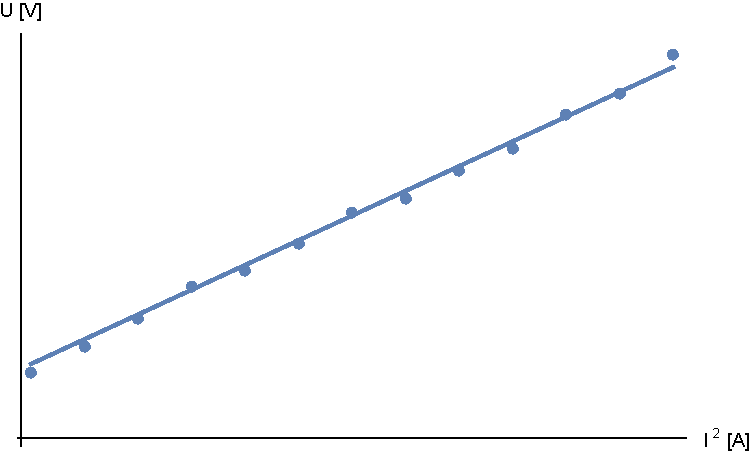
\includegraphics[width=0.7\linewidth]{wyk1}
\caption{Płytki odległe od ekranu o 83 mm}
\label{fig:wyk1}
\end{figure}
\begin{figure}[h]
	\centering
	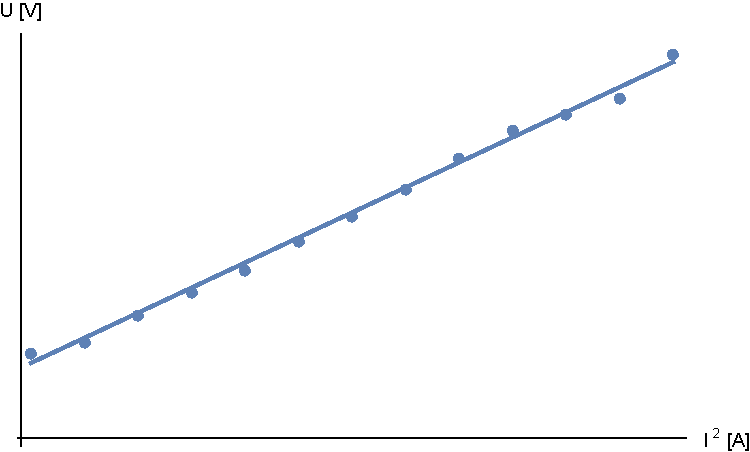
\includegraphics[width=0.7\linewidth]{wyk2}
	\caption{Płytki odległe od ekranu o 102 mm}
	\label{fig:wyk2}
\end{figure}
\subsection{Przypadek pola poprzecznego}
\subsubsection{Poprzeczne pole elektryczne}
Zakładamy następujące warunki układu:
\begin{align*}
\vec{v}=(v,0,0),\qquad \vec{E}=(0,-E,0),\qquad\vec{B}=0
\end{align*}
Wtedy w kierunku osi $Ox$ elektrony poruszają się ze stałą prędkością i są przyspieszane w kierunku osi $Oy$. Po opuszczeniu kondensatora poruszają się ruchem jednostajnym ze składowymi w $Ox$ i $Oy$. Możemy wyliczyć prędkość i odległość jaką przebyły elektrony w obszarze kondensatora:
\begin{align*}
a_y=-\frac{e}{m}(-E)
\end{align*}
Co daje nam prędkość jaką uzyskał elektron:
\begin{align*}
v_y=\frac{eE}{m}t\\
y=\frac{eE}{2m}t^2
\end{align*}
Biorąc pod uwagę, że w tym samym czasie elektron przebył długość kondenastora w kierunku $Ox$, to $t=\frac{d}{v}$, co nam daje:
\begin{align*}
v_y=\frac{eE}{m}\frac{d}{v}\\
y=\frac{eE}{2m}\frac{d^2}{v^2}
\end{align*}
W dalszej części układu mamy wiazkę poruszającą sie ze stałymi prędkościami, więc dostajemy równiania:
\begin{align*}
x=d+vt'\\
y=\frac{eE}{2m}\frac{d^2}{v^2}+\frac{eE}{m}\frac{d}{v}t'
\end{align*}
Ale ponownie możemy zauważyć, że w czasie $t'$ wiązka przebywa odległość $l-d$ od kondensatora do ekranu, więc $t'=\frac{l-d}{v}$, co daje nam:
\begin{align*}
y=\frac{eE}{2m}\frac{d^2}{v^2}+\frac{eE}{m}\frac{d}{v}\frac{l-d}{v}=\frac{eE}{m}\frac{d}{v^2}\left(\frac{d}{2}+l-d\right)=
\frac{eE}{m}\frac{d}{v^2}\left(l-\frac{d}{2}\right)
\end{align*}
Biorąc pod uwagę, ze pole możemy wyznaczyć jako $E=\frac{U}{s}$:
\begin{align*}
y=\frac{eU}{sm}\frac{d}{v^2}\left(l-\frac{d}{2}\right)
\end{align*}
Przekształcając do wyrażenia na ładunek właściwy:
\begin{align*}
\frac{e}{m}=\frac{ysv^2}{Ud}\left(l-\frac{d}{2}\right)^{-1}
\end{align*}
Gdzie zgodnie z intrukcją stanowiska wartości poszczególnych parmetrów układu wynoszą:
\begin{itemize}
	\item Nominalna prędkość wiązki: $v=102.7\cdot 10^5\:\mathrm{\frac{m}{s}}$
	\item Długość układu: $l=0.09\:\mathrm{m}$
	\item Dlugość okładek rozchylających: $d=0.011\:\mathrm{m}$
	\item Odległość pomiędzy okładkami rozchylającymi: $s=0.004\:\mathrm{m}$
\end{itemize}
Mamy $8$ zestawów danych, licząc wartości $e/m$ dla każdego i wyciągając średnią:
\begin{align}
\frac{e}{m}=2.08479\cdot10^{11}\:\mathrm{\frac{C}{kg}}
\end{align}
\subsubsection{Poprzeczne pole magnetyczne}
Analogicznie do poprzedniego przykładu odchylenie ma postać:
\begin{align*}
y=\frac{2Beb}{vm}\left(l-\frac{b}{2}\right)=\left(\frac{4}{5}\right)^\frac{3}{2}\frac{2\mu_0nI}{R}\frac{eb}{vm}\left(l-\frac{b}{2}\right)
\end{align*}
Gdzie parametry nie występujące w poprzednim paragrafie to:
\begin{itemize}
	\item Długość obszaru pola magnetycznego: $b=0.011\:\mathrm{m}$	
	\item Promień cewki: $R=0.05\:\mathrm{m}$
	\item Stała przenikalności magnetycznej: $\mu_0=1.256\cdot10^{-6}\:\frac{\mathrm{Vs}}{\mathrm{Am}}$
	\item Liczba zwojów na cewce $n=650$
\end{itemize}
Czyli przekształcając do postaci na ładunek właściwy:
 \begin{align*}
 \frac{e}{m}=\left(\frac{4}{5}\right)^{-\frac{3}{2}}\frac{Rv}{2In\mu_0b}\left(l-\frac{b}{2}\right)^{-1}
 \end{align*}
 Średnia z naszego zestawu danych to:
 \begin{align}
 \frac{e}{m}=1.14047\cdot10^{11}\:\mathrm{\frac{C}{kg}}
 \end{align}
\subsection{Metoda Thompsona}
\subsubsection{Wyznaczenie prędkości wiązki}
Wiemy, że by wiązka elektornowa ogniskowała się na środku ekranu musi zachodzić równowaga sił elektrycznej i magnetycznej:
\begin{align*}
eE=evB\qquad\Rightarrow \qquad v=\frac{E}{B}
\end{align*}
Gdzie $B=\left(\frac{4}{5}\right)^\frac{3}{2}\frac{\mu_0I}{R}$, a $E=\frac{U}{d}$. Dostajemy wyrażenie, dzięki któremu możemy wyznaczyć prędkość wiązki elektronów:
\begin{align*}
v=\frac{UR}{d\mu_0nI}\left(\frac{4}{5}\right)^\frac{3}{2}
\end{align*}
Mamy $8$ zestawów danych. Licząc średnią z nich wszystkich otrzymujemy 
\begin{align*}
v=8.82786\cdot10^6\:\mathrm{\frac{m}{s}}.
\end{align*}
\subsubsection{Pole elektryczne}
W tym przypadku obliczamy ładunek właściwy analogicznie do przypadku pola poprzecznego, tylko jako prędkość wiązki przyjmujemy wartość wyliczoną w paragrafie $5.3.1$.
Korzystamy ze wzoru:
\begin{align*}
\frac{e}{m}=\frac{ysv^2}{Ud}\left(l-\frac{d}{2}\right)^{-1}
\end{align*}
Dla naszego zestawu danych otrzymujemy:
\begin{align}
\frac{e}{m}=1.55836\cdot10^{11}\:\mathrm{\frac{C}{kg}}
\end{align}
\subsubsection{Pole magnetyczne}
W tym przypadku obliczamy ładunek właściwy analogicznie do przypadku pola poprzecznego, tylko jako prędkość wiązki przyjmujemy wartość wyliczoną w paragrafie $5.3.1$.
Korzystamy ze wzoru:
 \begin{align*}
 \frac{e}{m}=\left(\frac{4}{5}\right)^{-\frac{3}{2}}\frac{Rv}{2In\mu_0b}\left(l-\frac{b}{2}\right)^{-1}
 \end{align*}
 Dla naszego zestawu danych otrzymujemy:
 \begin{align}
 \frac{e}{m}=1.52021\cdot10^{11}\:\mathrm{\frac{C}{kg}}
 \end{align}
 \subsubsection{Podsumowanie Methody Thompsona}
 Teraz ponieważ wyniki dla obu pól były otrzymywane w sposób skorelowany, to wyciągniemy średnią z ich wartości:
 \begin{align}
 \frac{e}{m}=\left(\frac{1.52021+1.55836}{2}\right)\cdot10^{11}\:\mathrm{\frac{C}{kg}}=1.53928\cdot10^{11}\:\mathrm{\frac{C}{kg}}
 \end{align}
\section{Ocena niepewności}
By obliczyć niepewność naszych pomiarów zastosujemy niepewność standardową, która jest postaci:
\begin{align}
u(a)=\sqrt{\frac{1}{n(n-1)}\sum\limits_{i=1}^{n}\left(a_i-\bar{a}\right)^2}
\end{align}
\subsection{Podłużne pole}
\begin{align*}
u\left(\frac{e}{m}=1.54979\cdot10^{11}\right)=1.43231\cdot10^9=0.014\cdot10^{11}
\end{align*}
\subsection{Poprzeczne pole}
\subsubsection{Pole elektryczne}
\begin{align*}
u\left(\frac{e}{m}=2.08479\cdot10^{11}\right)=3.65962\cdot10^9=0.037\cdot10^{11}
\end{align*}
\subsubsection{Pole magnetyczne}
\begin{align*}
u\left(\frac{e}{m}=1.14047\cdot10^{11}\right)=5.46617\cdot10^{9}=0.055\cdot10^{11}
\end{align*}
\subsection{Metoda Thompsona}
\subsubsection{Niepewność prędkości}
\begin{align*}
u\left(v=8.82786\cdot10^6\right)=2.06156\cdot10^5=0.2\cdot10^6
\end{align*}
\subsubsection{Niepewność pomiaru}
\begin{align*}
u\left(\frac{e}{m}=1.53928\cdot10^{11}\right)=1.63533\cdot10^9=0.016\cdot10^{11}
\end{align*}
\section{Wnioski}
Zgodnie z danymi tabelarycznymi ładunek właściwy wynosi $\frac{e}{m}=1.758\cdot10^{11}\:\mathrm{\frac{C}{kg}}$[3].\\
Widzimy, że wartości przez nas uzyskane istotnie odbiegają od wartości rzeczywistych. Co mogło być tego przyczyną? Przyczyn mogło być wiele. Część z nich mogła być związana z dokładnością układu pomiarowego, jednak prawopodobnie większość niedokładności pomiaru było związane z błędami odczytowymi obserwatora.\\
 Przy pomiarze w polu podłużnym odczyt z ekranu był bardzo subiektywny. Trudno było ocenić, kiedy plamka osiąga minimu powierzchni. Pomimo tego widzimy, że pomiary zachowują charakter liniowy $U(I^2)$. \\
 W kolejnych pomiarach problemem mógł być błąd paralaksy, co mogło skutkować istotnymi odchyłami od wartości rzeczywistych. \\
 Podsumowując, z przybliżeniem do błędów eksperymentatora, uzyskaliśmy zadowalający wynik różniący się poniżej $40\%$ od wartości rzeczywistych.
\begin{thebibliography}{99}
	\bibitem{1}K. Sierański, K. Jezierski, B. Kołodka, \textit{ Wzory i prawa z objaśnieniami, cz. I}, Oficyna  Wydawnicza Scripta, Wrocław 2005
	\bibitem{2} D. Halliday, R. Resnick, J.Walker, \textit{Podstawy fizyki}, t.3 
	\bibitem{3}
	T. Szymczyk, \emph{Tablice matematyczne, fizyczne, astronomiczne i chemiczne}, PPU "PARK", Bielsko-Biała 2002
\end{thebibliography}
\end{document}